\section{Threshold expansion}
\label{sec:expansion}

\subsection{Construction}

After the substitution of Eq.~\eqref{eq:threshold-map}, each flavour coefficient is expanded at fixed $c$,
\begin{equation}
 \Mflav{i}{r}(\bA,c)
 =\sum_{n=-4}^{p}\sum_k
 C^{(i,r)}_{nk}\,\bA^n\ln^k\bA
 +\mathcal O_{\log}(\bA^{p+1}),
 \label{eq:series-structure}
\end{equation}
with $r=0,1,2$ and $p=4$ or 6. The coefficients $C^{(i,r)}_{nk}$ depend on $c$, $\mA^2$, $\muR^2$ and $\Nc$, and $\mathcal O_{\log}(\bA^n)$ stands for $\bA^n$ times a polynomial in $\ln\bA$. Inverse powers appear in intermediate steps because the tensor basis and the rational prefactors contain inverse Gram determinants, Eq.~\eqref{eq:gram-scaling}. They must be kept until all contributions at a given power have been combined.

The remainders contain logarithms, classical polylogarithms and the function $\Li_{2,2}$ of weight four~\cite{Frellesvig:2016ske,Vollinga:2004sn}, whose arguments approach correlated endpoints as $\bA\to0$. I expand the rational prefactors exactly and obtain the expansions of the special functions from differential equations in $\bA$, with boundary values at $\bA=0$. These equations have the iterated-integral form familiar from harmonic polylogarithms~\cite{RemiddiVermaseren2000} and from canonical differential equations for Feynman integrals~\cite{Henn2013}; the map $x=(1-\bA)/(1+\bA)$ is one of the transformations under which harmonic polylogarithms are closed~\cite{RemiddiVermaseren2000}. The method thus expands the known remainders, not the loop integrals, which could instead be expanded near threshold by the method of regions~\cite{BenekeSmirnov1998}. For the dilogarithm, for example, $\dd\Li_2(x)/\dd\bA=2(1-\bA^2)^{-1}\ln[2\bA/(1+\bA)]$ with $\Li_2(1)=\pi^2/6$ gives
\begin{align}
 \Li_2(x)
 &=
 \frac{\pi^2}{6}
 +2\bA\bigl[\ln(2\bA)-1\bigr]
 -\bA^2
 \nonumber\\
 &\quad
 +\bA^3
 \left[
   \frac{2}{3}\ln(2\bA)
   +\frac{1}{9}
 \right]
 -\frac{2}{3}\bA^4
 +\Ord\!\left(\bA^5\ln\bA\right).
 \label{eq:li2-threshold-example}
\end{align}
Since the prefactors start at $\bA^{-4}$, the special functions have to be expanded four orders beyond the final accuracy. The fourth and sixth order expansions were constructed independently, and all coefficients common to both agree.

\subsection{Endpoint constants and exact cancellations}
\label{sec:cancellations}
% Defined ahead of the citing text: a page-wide float can only appear at the top of a later page.
\begin{figure*}[t]
 \centering
 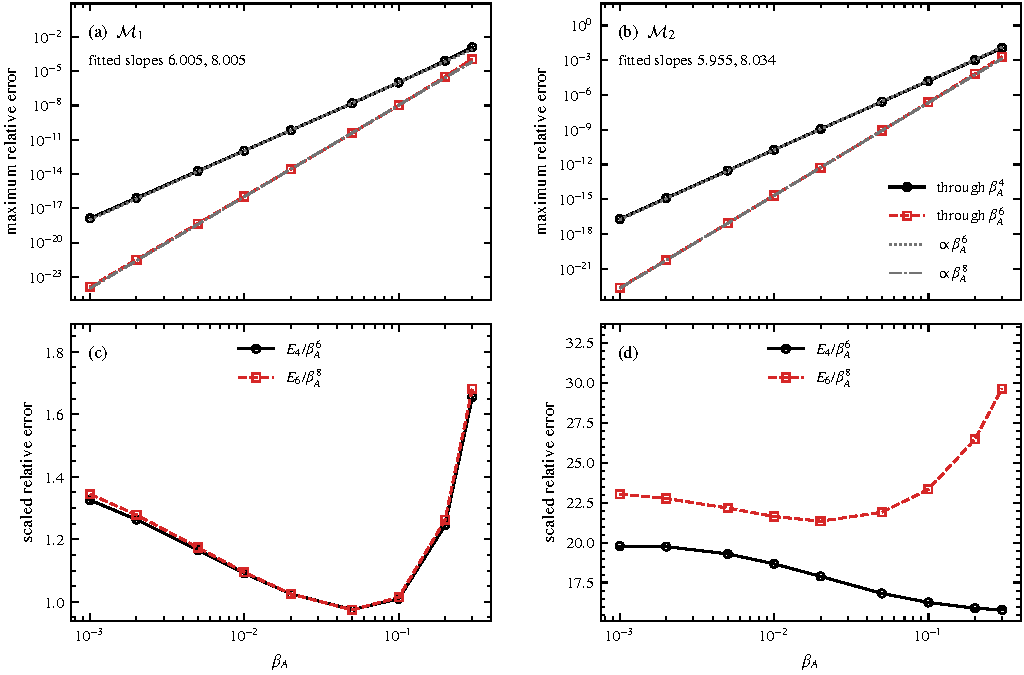
\includegraphics[width=0.98\textwidth]{figures/fig1_validation.pdf}
 \caption{Maximum relative errors of the complete two-loop coefficients after truncation at $\bA^4$ and $\bA^6$, with $\bA^6$ and $\bA^8$ for comparison (upper panels), and after division by these powers (lower panels). The maximum is taken over the five angles and three parameter sets of Table~\ref{tab:validation-grid}.}
 \label{fig:validation}
\end{figure*}


The boundary values at $\bA=0$ introduce \ConstantCountWord{} constants $\mathrm{MB}[p,q,a,w]$, defined in Eq.~\eqref{eq:mb-definition} of App.~\ref{app:constants}. Their arguments take the values $\pm1$ and $\tfrac12$, so they are alternating Euler sums of weight three and four~\cite{Blumlein:2009cf}. An integer relation search with the PSLQ algorithm~\cite{Ferguson:1999} at \PSLQDigits{} digits expresses each of them in the basis
\begin{equation}
 \{\zeta_3,\ \pi^2\ln2,\ \ln^32,\ \pi^4,\ \pi^2\ln^22,\ \ln^42,\ \Li_4(\tfrac12),\ \zeta_3\ln2\},
 \label{eq:constant-basis}
\end{equation}
with a largest residual of \PSLQResidual{} (Table~\ref{tab:mb-constants}).

With these reductions, and with the dilogarithms of $(1-c)/2$, $(c-1)/(c+1)$ and $(c+1)/(c-1)$ rewritten through $\Li_2\bigl((1+c)/2\bigr)$ by the reflection and Landen identities, every coefficient $C^{(i,r)}_{nk}$ becomes a polynomial in
\begin{equation}
 \bigl\{\ln\bA,\ \ln(1\pm c),\ \Li_2\bigl(\tfrac{1+c}{2}\bigr),\ \ln\tfrac{\mA^2}{\muR^2}\bigr\}\cup\{\ln2,\ \pi,\ \zeta_3,\ \Li_4(\tfrac12)\}
 \label{eq:function-basis}
\end{equation}
with coefficients rational in $c$ and $\Nc$. Treating these quantities as algebraically independent, I find that
\begin{enumerate}
 \item the coefficients of $\bA^{-4},\dots,\bA^{-1}$ vanish identically in every flavour coefficient;
 \item the coefficients of $\bA$, $\bA^3$ and $\bA^5$ vanish identically, so that through $\bA^6$ the expansion is a series in $\bA^2$ with logarithms;
 \item the coefficients of $\bA^0$, $\bA^2$, $\bA^4$ and $\bA^6$ of all six flavour coefficients, \LeadCheckedCount{} in total, are even in $c$, so that Bose symmetry holds order by order.
\end{enumerate}
The cancellations and the reductions of the constants were confirmed independently in Mathematica.

The cancellations have a simple origin. Exchanging the pseudoscalars exchanges $t$ and $u$, and the invariants that are symmetric under this exchange, $\hat s=4\mA^2/(1-\bA^2)$, $(t-u)^2=\hat s^2\bA^2c^2$ and $tu-\mA^4=\hat s\,p_T^2$ with $p_T^2=\hat s\bA^2(1-c^2)/4$, depend on $\bA$ only through $\bA^2$. No massive particle propagates in the loops, so the remainders are regular at $\hat s=4\mA^2$, and a colourless final state has no Coulomb singularity. Near threshold the only singularity is then the one at $p_T\to0$ discussed in Sec.~\ref{sec:dps}, which is logarithmic at one loop~\cite{GauntStirling2011}; the inverse Gram determinants of the tensor basis vanish at the same point but belong to the basis, not to the amplitude. A Bose symmetric function whose only singularity is logarithmic in $p_T^2$ is a series in $\bA^2$ with logarithms and has no inverse powers. At two loops this accounts for the cancellations found above but does not prove them, since there the logarithmic nature of the singularity is known only from the result itself. Table~\ref{tab:leading-threshold-inventory} lists the leading terms. Since the first omitted term is $\Ord_{\log}(\bA^{p+2})$, the truncation errors should scale as $\bA^6$ and $\bA^8$ for $p=4$ and 6.

\begin{table}[t]
\centering


\begin{tabular}{lccc}
\toprule
& inverse powers & leading & powers \\
quantity & in construction & power & of $\mathcal L$ \\
\midrule
$\Mflav{1}{0}$ & $\bA^{-2}$, $\bA^{-1}$ & $\bA^{0}$ & $0,1,2,3$ \\
$\Mflav{1}{1}$ & -- & $\bA^{0}$ & $0,1,2$ \\
$\Mflav{1}{2}$ & -- & $\bA^{0}$ & $0$ \\
$\Mflav{2}{0}$ & $\bA^{-4}$, $\bA^{-3}$, $\bA^{-2}$, $\bA^{-1}$ & $\bA^{0}$ & $0,1,2$ \\
$\Mflav{2}{1}$ & $\bA^{-1}$ & $\bA^{0}$ & $0,1$ \\
$\Mflav{2}{2}$ & -- & $\bA^{2}$ & $0$ \\
\bottomrule
\end{tabular}
\caption{Leading terms of the threshold expansion of the two-loop Type II remainders. The second column lists the inverse powers with nonzero coefficients in the construction files; they cancel identically after the reductions of Sec.~\ref{sec:cancellations}, as do all odd powers. The last column gives the powers of $\mathcal L$, Eq.~\eqref{eq:calL}, at leading power.}
\label{tab:leading-threshold-inventory}
\end{table}


The coefficient of $\nf^2$ is the simplest:
\begin{align}
 \Mflav{1}{2}(\bA,c)&=K+\Ord(\bA^2),
 \label{eq:nf2-leading-one}\\
 \Mflav{2}{2}(\bA,c)&=\bA^2(1-c^2)K+\Ord(\bA^4),
 \label{eq:nf2-leading-two}
\end{align}
where $K$ does not depend on the angle. It is the only flavour coefficient that follows the tree-level pattern $\mathcal M_2\propto\bA^2(1-c^2)$ of Eq.~\eqref{eq:born}, with the same ratio to the tree amplitude in both tensor structures. The complete expressions through $\bA^6$ are released as Wolfram Language files (App.~\ref{app:data}).

\subsection{Accuracy}
\label{sec:validation}

I compared the series with the unexpanded remainders at \BetaPointCount{} values of $\bA$ between \ValBetaMin{} and $\ValBetaMax$, \AnglePointCount{} angles and \ParameterSetCount{} choices of mass, scale and colour (Table~\ref{tab:validation-grid}). At each of the \GridPointCount{} points the test covers the six flavour coefficients and the two complete coefficients, \ValidationRows{} comparisons in total. Each unexpanded value is evaluated at increasing working precision until its real and imaginary parts are stable. The parameter set with $\Nc\neq3$ tests the colour dependence; all physical results use $\Nc=\BenchNc$. With the relative truncation error
\begin{equation}
 E_i^{(p)}
 =
 \frac{\left|\mathcal M_i^{[p]}-\mathcal M_i\right|}
      {\left|\mathcal M_i\right|},
 \qquad p=4,6,
 \label{eq:relative-error}
\end{equation}
where $\mathcal M_i$ is the unexpanded remainder and $\mathcal M_i^{[p]}$ its series through $\bA^p$. Fig.~\ref{fig:validation} shows the maximum over angles and parameter sets at each $\bA$. Fits give $E^{(4)}_i\propto\bA^{\PoneSlopeFour}$ and $\bA^{\PtwoSlopeFour}$, and $E^{(6)}_i\propto\bA^{\PoneSlopeSix}$ and $\bA^{\PtwoSlopeSix}$, as expected for a series in $\bA^2$. The lower panels divide out these powers. The ratios vary only slowly with $\bA$, because the first omitted coefficient contains powers of $\ln\bA$, and change most near $\bA=\EdgeBeta$, where the next order is no longer negligible; an error at a lower order would make them grow as an inverse power of $\bA$. For $\bA\leq\RecommendedBeta$ the sixth order series reproduces the complete coefficients with relative errors of at most \PoneErrLePointTwo{} and \PtwoErrLePointTwo; at $\bA=\EdgeBeta$ the errors are \PoneErrAtPointThree{} and \PtwoErrAtPointThree{} (Table~\ref{tab:AA-threshold-accuracy}). The values at $c$ and $-c$ \BoseStatement, in \AngularReferenceChecks{} comparisons of the unexpanded coefficients and \AngularSeriesChecks{} of the series.

\begin{table}[t]
\centering
\caption{Validation grid. At each point the six flavour coefficients and the two complete $\nf=\BenchNf$ coefficients are compared.}
\label{tab:validation-grid}
\begin{ruledtabular}
\begin{tabular}{ll}
quantity & values \\
\hline
$\bA$ & $1/1000$, $1/500$, $1/200$, \\
 & $1/100$, $1/50$, $1/20$, \\
 & $1/10$, $1/5$, $3/10$ \\
$c$ & $-2/3$, $-1/3$, $0$, $1/3$, $2/3$ \\
$(\mA/\mathrm{GeV},\,\muR/\mathrm{GeV},\,\Nc)$ & $(125,125,3)$, \\
 & $(125,250,3)$, \\
 & $(150,75,4)$ \\
\end{tabular}
\end{ruledtabular}
\end{table}


\begin{table}[!htb]
\centering
\caption{Maximum relative errors of the complete Type II coefficients on the validation grid. At each value of $\beta_A$, the maximum is taken over the \AnglePointCount{} angles and \ParameterSetCount{} parameter sets of Table~\ref{tab:validation-grid}.}
\label{tab:AA-threshold-accuracy}
\small
\setlength{\tabcolsep}{3pt}
\begin{ruledtabular}
\begin{tabular}{ccccc}
 & \multicolumn{2}{c}{$\mathcal{M}_1$ through} & \multicolumn{2}{c}{$\mathcal{M}_2$ through} \\
$\beta_A$ & $\beta_A^4$ & $\beta_A^6$ & $\beta_A^4$ & $\beta_A^6$ \\
\hline
0.01 & $1.09\times 10^{-12}$ & $1.09\times 10^{-16}$ & $1.87\times 10^{-11}$ & $2.16\times 10^{-15}$ \\
0.05 & $1.52\times 10^{-8}$ & $3.81\times 10^{-11}$ & $2.63\times 10^{-7}$ & $8.55\times 10^{-10}$ \\
0.10 & $1.01\times 10^{-6}$ & $1.01\times 10^{-8}$ & $1.63\times 10^{-5}$ & $2.33\times 10^{-7}$ \\
0.20 & $7.97\times 10^{-5}$ & $3.23\times 10^{-6}$ & $1.02\times 10^{-3}$ & $6.77\times 10^{-5}$ \\
0.30 & $1.21\times 10^{-3}$ & $1.10\times 10^{-4}$ & $1.15\times 10^{-2}$ & $1.94\times 10^{-3}$ \\
\end{tabular}
\end{ruledtabular}
\end{table}


The reference values were computed in Mathematica from the published expressions. I also evaluated these expressions with an independent code written in Python with mpmath~\cite{mpmath}, which has its own reader of the published files and computes $\Li_{2,2}$ from its defining double sum, with a one-dimensional integral representation where the sum converges slowly. At \ExactPointCount{} points covering the \ExactParameterSets{} parameter sets, the two complete coefficients agree with the reference values to a relative difference of at most \ExactMaxComplete, the precision to which the latter are stored; the \ExactComponentCount{} flavour coefficients at $\bA=\ExactComponentBeta$, $c=\ExactComponentCos$ agree to \ExactMaxComponent. The published expressions contain removable singularities at $c=0$, where $t=u$, which have to be taken as limits.

The expansion is carried out at fixed angle, but $p_T$ also vanishes when $c\to\pm1$ at fixed $\bA$. I therefore extended the comparison to $c=$ \ForwardCosList{} at $\bA=$ \ForwardBetaList{} (Table~\ref{tab:forward-angles}). \ForwardSummary{} The series thus remains accurate close to the beam, consistent with the absence of poles at $c=\pm1$ in its coefficients (Sec.~\ref{sec:leading}).

\begin{table}[t]
\centering
\caption{Relative truncation errors $E_i^{(6)}$ of the complete $\nf=\BenchNf$ coefficients towards the beam, at $\mA=\muR=\BenchMA\,\mathrm{GeV}$ and $\Nc=\BenchNc$. The last rows give the largest value on the grid of Table~\ref{tab:validation-grid}. The values at $c=-0.99$ equal those at $-c$.}
\label{tab:forward-angles}
\begin{ruledtabular}
\setlength{\tabcolsep}{3pt}
\begin{tabular}{llccc}
 & $c$ & $\bA=0.1$ & $\bA=0.2$ & $\bA=0.3$ \\
\hline
$\mathcal M_1$ & $0.9$ & $6.36\times10^{-9}$ & $1.11\times10^{-6}$ & $1.78\times10^{-5}$ \\
$\mathcal M_1$ & $0.99$ & $1.06\times10^{-8}$ & $2.43\times10^{-6}$ & $5.76\times10^{-5}$ \\
$\mathcal M_1$ & $0.999$ & $1.23\times10^{-8}$ & $2.96\times10^{-6}$ & $7.18\times10^{-5}$ \\
$\mathcal M_2$ & $0.9$ & $1.39\times10^{-7}$ & $3.08\times10^{-5}$ & $6.68\times10^{-4}$ \\
$\mathcal M_2$ & $0.99$ & $6.68\times10^{-8}$ & $1.47\times10^{-5}$ & $2.88\times10^{-4}$ \\
$\mathcal M_2$ & $0.999$ & $6.21\times10^{-8}$ & $1.65\times10^{-5}$ & $3.74\times10^{-4}$ \\
$\mathcal M_1$ & grid max. & $1.01\times10^{-8}$ & $3.23\times10^{-6}$ & $1.10\times10^{-4}$ \\
$\mathcal M_2$ & grid max. & $2.33\times10^{-7}$ & $6.77\times10^{-5}$ & $1.94\times10^{-3}$ \\
\end{tabular}
\end{ruledtabular}
\end{table}

